%% -*- LaTeX -*- This is LaTeX2e code

\documentclass{article}

\usepackage{amsmath}
\usepackage{algorithm}
\usepackage{algorithmic}
\usepackage{verbatim}

%
%  See whether we're running pdflatex (from pdflatex FAQ).
%

\newif\ifpdf
\ifx\pdfoutput\undefined
  \pdffalse
\else
  \pdfoutput=1
  \pdftrue
\fi

%
%  Setup graphics and pdfinfo/pdfcatalog.
%

\ifpdf
  \usepackage[pdftex]{graphicx}
  \DeclareGraphicsExtensions{.pdf}
  \pdfcompresslevel=9
  \pdfinfo {
    /Title       (Space-Efficient Geometric Divide-and-Conquer Algorithms)
    /Creator     (LaTeX)
    /Producer    (pdfTeX (Web2C 7.3) 3.14159-0.13c)
    /Author      (Prosenjit Bose, Anil Maheshwari, Pat Morin, Jason Morrison, Michiel Smid, Jan Vahrenhold)
    /Subject     ()
    }
  \pdfcatalog {
    /PageMode /UseNone
    }
\else
  \usepackage{graphicx}
  \DeclareGraphicsExtensions{.eps}
\fi

%%
%%  Some macros.
%%

%% Complexity of algorithms
\newcommand{\Oh}[1]{\ensuremath{\mathcal{O}(#1)}}
\newcommand{\Wm}[1]{\ensuremath{\Omega(#1)}}
\newcommand{\orderof}[1]{\ensuremath{\Theta(#1)}}
\def\bbbn{{\rm I\!N}}

\def\etal{\textit{et~al.}}

\newcommand{\set}{\ensuremath{\mathcal{S}}}

\newcommand{\graphicxbox}[2]{\centerline{\includegraphics[width=#1]{#2}}}
\newcommand{\graphicybox}[2]{\centerline{\includegraphics[height=#1]{#2}}}

%%
%%  End of "Some macros."
%%

%%
%%  Macro for writing in the margin comments on what is left to be done.
%%

\newif\ifdraft
                \drafttrue
                %\draftfalse

\ifdraft
\addtolength{\oddsidemargin}{-0.5 in}
\addtolength{\evensidemargin}{+0.5 in}
\newcounter{ournotecounter}
\newcommand{\ournote}[1]{%
  \refstepcounter{ournotecounter}%
  \ifhmode%
  \unskip%
  {\dimen1=\baselineskip \divide\dimen1 by 2 %
    \raise\dimen1\llap{\tiny -\theournotecounter-}}\fi%
  \marginpar{\renewcommand{\baselinestretch}{0.8}%
    \footnotesize [\theournotecounter]: \raggedright #1}}
\newcommand{\longnote}[1]{\fbox{\parbox{0.9\textwidth}{#1}}}
\typeout{Compiling in draft mode.}
\else
\newcommand{\ournote}[1]{}
\newcommand{\longnote}[1]{}
\typeout{Compiling in final mode.}
\fi

\newtheorem{theorem}{Theorem}
\newtheorem{lemma}{Lemma}
\newtheorem{definition}{Definition}

%%
%%  End of macro.
%%

\usepackage{fullpage}
\begin{document}

%% -*- LaTeX -*- This is LaTeX2e code

\title{Space-Efficient Geometric Divide-and-Conquer Algorithms}

\author{%
Prosenjit Bose\thanks{School of Computer Science, Carleton
    University, 1125 Colonel By Dr., Ottawa, Ontario, Canada, K1S~5B6.
    Email: \texttt{\{jit, anil, morin, morrison, michiel\}@scs.carleton.ca}. Research supported in part by NSERC.} 
\and Anil Maheshwari\footnotemark[1]
\and Pat Morin\footnotemark[1]
\and Jason Morrison\footnotemark[1]
\and Michiel Smid\footnotemark[1]
\and Jan
  Vahrenhold\thanks{Westf\"{a}lische Wilhelms-Universit\"{a}t,
    Institut f\"{u}r Informatik, 48149 M\"{u}nster, Germany.  Email:
    \texttt{jan@math.uni-muenster.de}. Part of this work was done
    while visiting Carleton University.  Supported in part by DAAD
    grant D/0104616.  } }

\ifdraft
\date{Draft as of \today}
\fi

%%% Local Variables:
%%% mode: latex
%%% TeX-master: "paper"
%%% End:


\maketitle

%% -*- LaTeX -*- This is LaTeX2e code


\begin{abstract}
We develop a number of space-efficient tools including an approach to
simulate divide-and-conquer space-efficiently, stably selecting and
unselecting a subset from a sorted set, and computing the $k$th
smallest element in one dimension from a multi-dimensional set that is
sorted in another dimension.  We then apply these tools to solve
several geometric problems that have solutions using some form of
divide-and-conquer. Specifically, we present solutions running in
\Oh{n \log n} time using \Oh{1} extra memory given inputs of size $n$
for the closest pair problem and the bichromatic closest pair 
problem.  For the orthogonal line segment intersection problem, we
solve the problem in \Oh{n\log n + k} time using \Oh{\log n} extra
space where $n$ is the number of horizontal and vertical line segments
and $k$ is the number of intersections.
\end{abstract}


%%% Local Variables:
%%% mode: latex
%%% TeX-master: "paper"
%%% End:


%% -*- LaTeX -*- This is LaTeX2e code



\section{Introduction}

Researchers have studied space-efficient algorithms since the early
70's. Examples include merging, (multiset) sorting, and partitioning
problems;
see~\cite{geffert:merging,katajainen:multisets,katajainen:partitioning}.
Br\"onnimann \etal~\cite{bronnimann:convex} were the first to consider
space-efficient geometric algorithms and showed how to compute the
convex hull of a planar set of $n$ points in \Oh{n \log h} time using
\Oh{1} extra space, where $h$ denotes the size of the output.
Recently, Chen and Chan~\cite{chen:space-efficient} addressed the
problem of computing the intersections among $n$ line segments, giving
an algorithm that runs in \Oh{(n+k)\log^2 n} time using \Oh{\log^2n}
extra space where $k$ is the number of intersections and an algorithm
that runs in \Oh{(n+k)\log n} time using \Oh{1} extra space but the
initial input is destroyed.  Br\"onnimann, Chan and
Chen~\cite{bronnimann:inplace} developed some space efficient data
structures and used them to solve a number of geometric problems such
as convex hull, Delaunay triangulation and nearest neighbor queries.
In this paper, we develop a number of space-efficient tools outlined
in Section \ref{sec:tools} that are of interest in their own right. We
then apply these tools to several geometric problems that have
solutions using some form of divide-and-conquer. Specifically, we
address the problems of closest pairs, bichromatic closest pair 
and orthogonal line segment intersection.

\ournote{Jit:  Can you please add a sentence for Br\"onnimann \etal~\cite{bronnimann:inplace}? I forgot my proceedings at home.}

\subsection{The Model}

The goal is to design algorithms that use very little extra space over
and above the space used for the input to the algorithm. The input is
assumed to be stored in an array of size $n$, thereby allowing random
access.  The specifics of the input are outlined with each problem
addressed.  We assume that a constant size memory can hold a constant
number of words. Each word can hold one pointer, or an \Oh{\log n} bit
integer, and a constant number of words can hold one element of the
input array. The extra memory used by an algorithm is measured in
terms of the number of extra words. In certain cases, the output may
be much larger than the size of the input. For example, given a set of
$n$ line segments, if the goal is to output all the intersections,
there may be as many as \Wm{n^2}. In such cases, we consider the
output memory to be write-only space usable for output but cannot be
used as extra storage space by the algorithm.  This model has been
used by Chen and Chan~\cite{chen:space-efficient} for variable size
output, space-efficient algorithms and accurately models algorithms
that have output streams with write-only buffer space.

The remainder of the paper is organized as follows. In Section
\ref{sec:tools}, we outline the space-efficient tools that will be
useful in the solution of the geometric problems addressed. In Section
\ref{sec:nn}, we present an \Oh{n \log n} time algorithm to solve the
closest pair problem using only \Oh{1} extra memory. In the following
subsection, we solve the bichromatic closest pair problem in \Oh{n
\log n} time using only \Oh{1} extra memory. The solution is
randomized but the extra memory used is still \Oh{1} in the worst
case.  Section \ref{sec:orth} presents a solution to the orthogonal
line segment intersection problem in \Oh{n\log n + k} time using
\Oh{\log n} extra space where $n$ is the number of line segments, and
$k$ is the number of intersections.  Finally, conclusions and open
problems are in Section \ref{sec:conc}.


%\begin{definition}
%  An algorithm that needs \Oh{1} extra working space is called
%  \emph{in-place}, and an algorithm that needs \Oh{\log_2 n} extra
%  space is called \emph{in situ}.
%\end{definition}
%
%Recently, Raman~\etal~\cite{raman:dynamic,raman:indexable} considered 
%\emph{succinct} representations of ordered sets that allowed for
%various dictionary operations.
%
%%% Local Variables:
%%% mode: latex
%%% TeX-master: "paper"
%%% End:



%% -*- LaTeX -*- This is LaTeX2e code

\section{Space-Efficient Tools} \label{sec:tools}
In this section, we outline a number of tools that will be useful in the sequel.

\subsection{Space-Efficient Divide-and-Conquer}\label{sec:dc}


In this subsection, we describe a simple scheme for space-efficiently
performing divide-and-conquer. In a standard recursive procedure, prior to each
recursive call, the current state of the procedure (i.e. the state of the
variables, program counter, etc.)  that is invoking the recursive call
is saved on a stack.  The variables making up the current state are
often referred to as the {\em activation frame} and the stack is
usually called the {\em recursion stack}. According to our model, a
constant amount of memory is sufficient to store one activation frame on
the recursion stack. Thus, in the standard recursive approach, the
amount of extra space needed for the recursion stack is directly
related to the height of the recursion tree.

In most divide-and-conquer situations, the recursion tree is balanced,
implying that only \Oh{\log n} extra space is needed for maintaining
the recursion stack when the input has size $n$.  In randomized
algorithms, such as Quicksort, the recursion tree can have linear
height in the worst case. However, by always recursing on the smaller
sub-array first\footnote{This is sometimes referred to as optimizing
tail recursion.}, a worst case size of \Oh{\log n} for the stack can
be maintained\cite{huang:one-way,wegner:generalized}.  Consider
Algorithm \ref{alg:recurse} below, which represents a generic template
for divide-and-conquer algorithms.  Note that ``PROCESS x" simply
refers to a set of non-recursive statements.


\begin{algorithm}
  \caption{\textsc{Recursive}($b,e$): Standard template for recursion}
  \label{alg:recurse}
  \begin{algorithmic}[1]
    \IF{$e-b < s$ where $s$ is the size of the recursion base.}
    \STATE \{PROCESS 1: Base instance operations.\}
    \ELSE
    \STATE \{PROCESS 2: Computations to partition the array $A[b,\ldots,e-1]$\}
    \STATE \textsc{Recursive}($b,\lfloor e/2 \rfloor$)
    \STATE \textsc{Recursive}($\lfloor e/2 \rfloor + 1,e$)
    \STATE \{PROCESS 3: Pre-merge operations\}
    \STATE Merge $A[b,\lfloor e/2 \rfloor-1]$ with $A[\lfloor e/2
\rfloor + 1,e-1]$.
    \STATE \{PROCESS 4: Post-merge operations\}
    \ENDIF
  \end{algorithmic}
\end{algorithm}

Can a balanced recursion tree arising from the above recursive
algorithm be traversed with only \Oh{1} extra memory as opposed to the
\Oh{\log n} extra memory used for the stack?  Our technique outlines a
method for converting any algorithm fitting the above recursive
template into one that uses only \Oh{1} extra memory. The recursion
tree is traversed in the same manner without use of the recursion
stack. In many cases, the same type of result can be obtained using
bottom-up merge, however, it is well known that bottom-up merge has
poor performance in the presence of caches.

The main idea (which is probably folklore, even though we have not
seen it explicitly in the literature) is to simulate a post-order
traversal of the recursion tree. We assume for simplicity that the
data to be processed is stored in an array $A=A[0,\ldots,n-1]$ of size
$n = 2^k$ for some positive integer $k$. The recursion tree
corresponding to the above divide-and-conquer scheme is a perfectly
balanced binary tree, in which each node at depth $0 \leq i < k$
corresponds to a subarray of the form $A[j \cdot 2^{k-i} ,\ldots, (j +
1) \cdot 2^{k-i} - 1]$ for some integer $0 \leq j \leq i$.\footnote{If
the problem size is not an exact power of two, we imagine the
recursion tree to be embedded into a perfectly balanced tree and stop
traversing the tree prematurely.}

Our scheme is presented in Algorithm~\ref{alg:traversal}. We maintain
two indices $b$ and $e$ that indicate the subarray $A[b ,\ldots, e-1]$
currently processed. We will use the binary representation of the
index $e$ to implicitly store the current status of the post-order
traversal, i.e., the node of the simulated recursion tree currently
visited.

\begin{algorithm}
  \caption{$\textsc{Stackless-Recursive}(b,e)$: Stackless simulation
of \textsc{Recursive}}
  \label{alg:traversal}
  \begin{algorithmic}[1]
    \STATE $b=0$ and $e=s$, $s$ is the size of the recursion base.
    \WHILE{$b\neq 0$ or $e\leq n$}
    \STATE \{PROCESS 1: Base instance operations. Process all items in
$A[b,\ldots, e-1]$.\}
    \STATE $i$ be the index of the least significant bit of $e$.
    \FOR{$c\gets 1,\ldots, i$}
    \STATE $b \gets e-2^c$.
    \STATE \{PROCESS 3: Pre-merge operations\}
    \STATE Merge  $A[b,\ldots, b+2^{c-1} - 1]$ with
$A[b+2^{c-1},\ldots, e-1]$
    \STATE \{PROCESS 4: Post-merge operations on $A[b,\ldots, e-1]$ \}
    \ENDFOR 
    %\STATE $b \gets e$.  Not needed because of line 7.
    \STATE $e \gets e + s$.
    \ENDWHILE
  \end{algorithmic}
\end{algorithm}

Determining the value of $i$ (Step 4) can be done in \Oh{1} amortized
time without extra space using a straightforward implementation of a
binary counter.  The above algorithm basically traverses the recursion
tree from left to right. When processing a leaf $v$, the algorithm
backtracks in geometrically increasing steps merging all subtrees
already traversed completely. This merging is done by traversing a
leaf-to-root path starting from $v$ but stopping as soon as the path
goes up to the right (Figure~\ref{fig:tree_spaceefficient}). The
correctness of the algorithm follows from the next
lemma\cite{cormen:alg}:

\begin{lemma}
  If the leaves of a complete binary tree are labeled from left to
  right (starting with $1$ for the leftmost leaf), the height of the
  largest subtree containing the leaf $e>1$ as its rightmost leaf is
  equal to the index $i$ of the least significant bit of the number
  $e$.
\end{lemma}

\begin{figure}
  \centerline{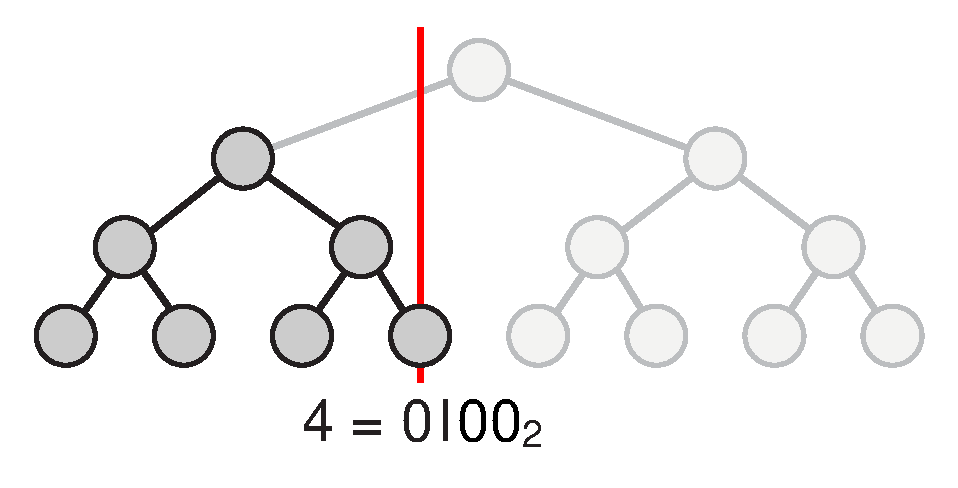
\includegraphics[height=3.5cm]{tree_spaceefficient}}
  \caption{Merging subtrees while traversing left-to-right.}
  \label{fig:tree_spaceefficient}
\end{figure}

Therefore, any algorithm that is in the form outlined by Algorithm
\ref{alg:recurse} using \Oh{\log n} extra space can be transformed
into a space-efficient algorithm of the form Algorithm \ref{alg:traversal}
using only \Oh{1} extra space provided that all the base instances
(i.e. leaves of the recursion tree) can be pre-computed with only \Oh{1} extra
space and PROCESS 1,3,4 as well as the Merge step can be made
space efficient using only \Oh{1} extra space. Note that PROCESS 2
operations no longer need to be computed in Algorithm \ref{alg:traversal}
since we assume that the array is initially partitioned into the
base instances. Therefore, there is no need to actually partition
the array as is done in PROCESS 2 in Algorithm \ref{alg:recurse}. Henceforth, we will refer
to recursive algorithms in standard form (i.e. Algorithm
\ref{alg:recurse}) as the {\em standard recursive form} and
space-efficient recursive algorithms (i.e. Algorithm \ref{alg:traversal})
as {\em space-efficient recursive form}. We conclude this section
with the following:

\begin{theorem}
An algorithm in standard recursive form running in \Oh{n \log n} time and using \Oh{\log n} extra space can be converted
to space-efficient recursive form running in \Oh{n \log n} time using only \Oh{1} extra space provided that all the base instances
(i.e. leaves of the recursion tree) can be pre-computed in \Oh{n \log n} time with only \Oh{1} extra
space and PROCESS 1,3,4 as well as the Merge step can be made
space efficient using only \Oh{1} extra space and \Oh{n} time.
\end{theorem}

Note that there can be trade-offs in the above theorem. For example, if in the space-efficient recursive form, the Merge step takes
\Oh{n \log n} time then, the overall running time becomes \Oh{n \log^2 n}. These trade-offs are fairly straightforward, related to the
Master Theorem for Recurrences \cite{cormen:alg} and can be adjusted to each situation.

\subsection{Sorted Subset Selection}

In this subsection, we introduce a simple yet surprisingly powerful
algorithm, called \textsc{SortedSubsetSelection}$(A,b,e,f)$.  The
algorithm provides a way of stably selecting a subset of the elements.
The key requirement is that the elements stored in the given array
$A[b,\ldots, e-1]$ are initially sorted according to some total order,
say $<_{A}$. The algorithm, described below as
Algorithm~\ref{alg:sortedSubsetSelection}, stably moves to the front
of the array all elements in $A[b,\ldots, e-1]$ for which the given
$(0,1)$-valued function $f$ returns the value one.  Moreover, this
algorithm has the desirable property that its effect can be reversed
easily.

\begin{algorithm}
  \caption{Algorithm
    $\textsc{SortedSubsetSelection}(A,b,e,f)$ for selecting a
    subset from a sorted array $A[b,\ldots, e-1]$.} 
  \label{alg:sortedSubsetSelection}
  \begin{algorithmic}[1]
    \REQUIRE Array $A[b,\ldots, e-1]$ is sorted according to
    some total order $<_{A}$, and $f$ is a 
    $(0,1)$-valued function that can be evaluated in constant
    time.
    
    \ENSURE $A[b,\ldots, m-1]$ contains all entries for which
    $f$ is one, and these entries are still (stably) ordered
    according to $<_{A}$.

    \STATE $i\gets b$, $j\gets b$ and $m\gets b+1$. 
    \WHILE{$i<e$ and $j<e$}
      \WHILE{$i<e$ and $f(A[i])=1$}
        \STATE $i\gets i+1$. \COMMENT{Move index $i$ such that
          $f(A[i])=0$.} 
      \ENDWHILE
      \STATE $j\gets i+1$;
      \WHILE{$(j<e)$ and $(f(A[j])=0)$}
        \STATE $j\gets j+1$. \COMMENT{Move index $j$ such that
        $f(A[j])=1$.} 
      \ENDWHILE
      \IF{$j<e$}
        \STATE Swap $A[i]$ and $A[j]$.
        \STATE $m\gets i+1$. \COMMENT{$A[b,\ldots, m-1]$
          contains all 1-valued entries.}
      \ENDIF
    \ENDWHILE
    \STATE Return $m$.
  \end{algorithmic}
\end{algorithm}

Algorithm~\ref{alg:sortedSubsetSelection} clearly uses only \Oh{1}
extra space and runs in linear time. The correctness of the algorithm
follows from the loop invariant that is maintained: $A[b,\ldots, m-1]$
stably contains all selected elements from $A[b,\ldots, e-1]$ whose rank
is at most $m-b$.  The effects of this algorithm can be reversed by
Algorithm~\ref{alg:revertSortedSubsetSelection}.

\begin{algorithm}
  \caption{Algorithm $\textsc{UndoSubsetSelection}(A,b,e,m)$
    for restoring the total order after applying the 
    \textsc{SortedSubsetSelection}-Algorithm~\ref{alg:sortedSubsetSelection}}
  \label{alg:revertSortedSubsetSelection}
  \begin{algorithmic}[1]

    \REQUIRE{Array $A[b,\ldots, m-1]$ contains the result of running
      Algorithm~\ref{alg:sortedSubsetSelection} on array
      $A[b,\ldots, e-1]$ that was sorted according to
      $<_{A}$.} 
    \ENSURE{Array $A[b,\ldots, e-1]$ is sorted according to
      $<_{A}$.} 
    \STATE $i\gets m-1$ and $j\gets e-1$.
    \WHILE{$i\neq j$ and $i\geq b$}
      \IF{$A[j]<_{A}A[i]$}
        \STATE Swap $A[i]$ and $A[j]$.
        \STATE $j\gets j-1$.
      \ENDIF
      \STATE $i\gets i-1$.
    \ENDWHILE

  \end{algorithmic}
\end{algorithm}

There is one important property to note:
Algorithm~\ref{alg:revertSortedSubsetSelection} does not require
knowledge of the selection function $f$, but only needs to know the
three indices $b$, $e$ and $m$. It only uses the order $<_{A}$ to
recover the state prior to the invocation of
\textsc{SortedSubsetSelection}. This is a key property that is useful
particularly if the selection function $f$ is unknown or cannot be
easily reconstructed.  In the following subsection, we show how useful
\textsc{SortedSubsetSelection} and its counterpart
\textsc{UndoSubsetSelection} are.


\subsection{Selecting the $k$-th smallest element}\label{sec:sel}

Selection of the $k$-th smallest element in-place is a fairly
difficult problem which makes use of stable partition which is
notoriously complicated\cite{kata:select}. However, in most geometric problems,
the input consists of a set of points in 2 or more dimensions.  If
the points are sorted with respect to one coordinate, selection of
the $k$-th smallest element with respect to another coordinate
becomes much easier.  We can take advantage of the total order in
one coordinate to simplify selection through the use of
SortedSubsetSelection. We outline a simple randomized algorithm
that runs in linear expected time and uses only \Oh{1} extra space.
Our algorithm is a slight modification of QuickSelect\cite{hoare:quicksort, cormen:alg}.


\begin{algorithm}
  \caption{Algorithm
    $\textsc{Select}(A,0,e,k)$ Select element in $A[0,e-1]$ with $k$-th smallest $X$-coordinate.}

  \label{alg:selectk}
  \begin{algorithmic}[1]
    \REQUIRE Array $A[0,\ldots, e-1]$ is sorted according to $Y$-coordinate.
    
    \ENSURE Element with $k$-th smallest $X$-coordinate is placed at
$A[0]$, and $A[1,\ldots, e-1]$ is sorted by $Y$-coordinate.

    \STATE $n \gets e$. \COMMENT{$n$ is the current size of the array being processed. }
    \WHILE{$n > 42$}
          \IF{k $< n/2$}
             \STATE Pick a random element $x$ whose rank is between $n/2$ and $3n/4$.
             \STATE Use \textsc{SortedSubsetSelection} to move all elements $< x$ and a sufficient number $> x$ to fill $A[0,\lfloor 3n/4 \rfloor - 1]$.
             \STATE Push $4(3n/4 - \lfloor 3n/4 \rfloor)$ on stack S.
             \STATE $n \gets \lfloor 3n/4 \rfloor$
          \ELSE
             \STATE Pick a random element $x$ whose rank is between $n/4$ and $n/2$.
             \STATE Use \textsc{SortedSubsetSelection} to move all elements $> x$ and a sufficient number $< x$ to fill $A[0,\lfloor 3n/4 \rfloor - 1]$.
             \STATE Push $4(3n/4 - \lfloor 3n/4 \rfloor)$ on stack S.
             \STATE $k \gets k - \lceil n/4 \rceil$.
             \STATE $n \gets \lfloor 3n/4 \rfloor$
          \ENDIF
    \ENDWHILE
    \STATE Find $k$-th smallest element in A[0,n-1] by brute force. $K
\gets$ this element.
    \STATE $M \gets n$
    \STATE $R \gets$ Pop top of stack.
    \STATE $D \gets (4M + R)/3$.
    \WHILE{$D < e$}
          \STATE UndoSubsetSelection($A,0,D,M$)
          \STATE $M \gets D$.
          \STATE $R \gets$ Pop top of stack.
          \STATE $D \gets (4M + R)/3$.
    \ENDWHILE
    \STATE Find $K$ in A[$0,\ldots, e-1$] and move it stably to A[$0$].
  \end{algorithmic}
\end{algorithm}

The main idea behind the algorithm is fairly simple. Refer to
Algorithm~\ref{alg:selectk}. If $k$ is smaller than $n/2$, then we
find an element $x$ whose rank is between $n/2$ and $3n/4$. The case
is similar if $k \geq n/2$. Since there are at least $n/4$ such
elements, with only an expected constant number of random selections,
we can find such an element.  Computing the rank of a given element
takes \Oh{n} time, thus in \Oh{n} expected time, we can find $x$. Note
that if we partition the array with $x$, then at least $n/4$ elements
can be eliminated.  The key is to eliminate {\em precisely} $n/4$
elements. This way, when it comes time to undo the operation, we know
exactly where the partition boundaries occur. This is where the stack
$S$ comes into play.  Each time through the loop, we reduce the size
of the array to $\lfloor 3n/4 \rfloor$. To undo this operation, we
need to record the actual remainder from the division by $3/4$. Two
bits are sufficient to record this since the remainder can only be one
of $\{0, 1, 2, 3\}$.  For example, suppose that the current instance
has an array of size 37.  Since $3\times 37/4 = 27+3/4$, the next
instance has size $27$ and we push the remainder $3$ on the stack.  In
the undo step, if the current instance is 27, to recover the size of
the array at invocation, we note that $(4*27 + 3)/3 = 37$ which is the
computation used to recover the indices required for the Undo
operation.

In the final loop where the steps are {\em undone}, the only
information we require are the three indices $0, D$ and $M$. We do not
need to remember the particular element $x$ that was used in the SortedSubsetSelection step. 
The sorted order on the $Y$-coordinate
is sufficient to recover the original order. 

Since at each iteration through the while loop, we eliminate
a quarter of the elements, the number of iterations through the loop is \Oh{\log n}. At
each iteration, two bits are pushed on the stack, so the total number of bits ever
stored in the stack is \Oh{\log n} which implies that only \Oh{1} extra space
is used. The running time of the algorithm is given by the following recurrence:
\[
T(n) = T(3n/4) + \Oh{n}
\] 
which resolves to \Oh{n}.

This algorithm can be made \Oh{n} deterministic. The only step where randomization is used is in the selection 
of the partition element $x$. In the deterministic version, we use techniques from 
the algorithm by Blum \etal~\cite{blum:selection}.
Instead of selecting an element at random, we select the partition element by first decomposing the
array into $n/5$ groups of 5 elements and computing the median of the medians of the groups. 
The idea is simple and similar to the above algorithm except some of the details are quite tedious, so we outline the details
in Appendix \ref{sec:detkmed}.





%%% Local Variables:
%%% mode: latex
%%% TeX-master: "paper"
%%% End:

% -*- LaTeX -*- This is LaTeX2e code

\section{Nearest Neighbor Problems}\label{sec:nn}

\subsection{Closest Pair}

Given a set $P$ of $n$ points in the plane stored in an array \texttt{A}$[0
\ldots n - 1]$, a closest pair is a pair of points in $P$ whose Euclidean
distance is smallest among all pairs of points. We modify an algorithm by
Bentley and Shamos~\cite{bentley:divide-and-conquer} to compute the closest
pair in \Oh{n \log n} time using only \Oh{1} extra space.

Algorithm~\ref{alg:bentley} describes a slightly modified version of Bentley's
divide-and-conquer algorithm for finding the closest pair.  The algorithm
works by drawing an imaginary vertical dividing line through the median
$X$-coordinate.  The algorithm then finds the closest pair with both points to
the left of this line, the closest pair with both points to the right of this
line and then finds the closest pair with one point on the left and one point
on the right of the line.  The first two closest pairs are computed with
recursive calls while the third closest pair is accomplished by a vertical
plane sweep of all the points that are ``close to'' the dividing line.
 
\begin{algorithm} \label{alg:nn}
  \caption{$\textsc{Nearest-Neighbor}(A,b,e)$: Divide-and-Conquer algorithm for finding a closest
    pair~\cite{bentley:divide-and-conquer}.} 
  \begin{algorithmic}[1]
    \REQUIRE All points in the input array $A$ are sorted according to
    $Y$-coordinate.
    \ENSURE The first two points in the array $A[b,\ldots,e-1]$ realize the closest pair and the remaining points are sorted by $Y$-coordinate.
    \IF{$e-b < 16$} 
      \STATE Compute a closest pair using a brute-force
algorithm, stably place them at the front of the current subarray and return.
    \ELSE
      \STATE Compute the median $X$-coordinate $x$ using
Algorithm~\ref{alg:selectk} (\textsc{Select}) while maintaining the array
sorted by $Y$-coordinate.
      \STATE Using Algorithm~\ref{alg:sortedSubsetSelection}, stably select all
elements of $A[b,\ldots,e-1]$ with $x$ coordinate less than or equal $x$ so
that they are stored in $A[b,\ldots,\lfloor e/2\rfloor-1]$. 
      \STATE \textsc{Nearest-Neighbor}($A,b,\lfloor e/2 \rfloor$)
      \STATE Using Algorithm~\ref{alg:revertSortedSubsetSelection}, restore
$A[b,\ldots,e-1]$ so that it is sorted by $Y$ coordinate.  Stably store the
closest pair from the previous step in $A[b]$ and $A[b+1]$.
       \STATE Using Algorithm~\ref{alg:sortedSubsetSelection}, stably select all elements of $A[b,\ldots,e-1]$ with $x$
coordinate greater than $x$ so that they are stored in
$A[\lfloor e/2\rfloor,\ldots,e-1]$. 
      \STATE \textsc{Nearest-Neighbor}($A,\lfloor e/2 \rfloor$,e)
       \STATE Using Algorithm~\ref{alg:revertSortedSubsetSelection}, restore
$A[b,\ldots,e-1]$ so that it is sorted by $Y$ coordinate.  Stably store the
closest pair from Step~6 or the closest pair from the previous step (whichever
is closer) at
locations $A[b]$ and $A[b+1]$.
      \STATE Let $\delta$ be the distance between $A[b]$ and $A[b+1]$.
      \STATE Using Algorithm~\ref{alg:sortedSubsetSelection}, extract in $Y$-sorted order the points of $A[b,\ldots,e-1]$ that fall within a
                strip of width $2\delta$ centered at the median $X$-coordinate of $A[b,\ldots,e-1]$.
         \STATE Scan the points in this strip to determine whether there is a pair of
                points with distance smaller than $\delta$. Update $\delta$ and
                the closest pair as necessary. 
        \STATE Using Algorithm~\ref{alg:revertSortedSubsetSelection}, restore
$A[b,\ldots,e-1]$ so that it is sorted by $Y$ coordinate.  Stably store the closest pair 
at
locations $A[b]$ and $A[b+1]$.
    \ENDIF
  \end{algorithmic}
\end{algorithm}

Note that the recursion tree for Bently and Shamos' algorithm is balanced
with the the two recursive calls occuring in lines 6 and 9 and that this
algorithm fits into the framework of the Algorithm~\ref{stackless}
(\textsc{Stackless-Recursive}).  In particular, PROCESS~1 takes place in
line~2, PROCESS~3 takes place in lines 


. For
simplicity of exposition, we stopped the recursion when an instance of size at
most 16 is reached.  Therefore, to apply our space-efficient recursion
template, we first need to show how to compute the base instances (i.e. leaves
of the recursion tree) and then elaborate on some of the details within the
PROCESSES.  The base of the recusion is trivially computed by running any
\emph{in-place} sorting algorithm, e.g., \emph{heapsort}~\cite{floyd:245}, to
sort the points according to their $X$-coordinate in \Oh{n \log n} time using
\Oh{1} extra space.

Now, to elaborate on the PROCESSES. First, steps in PROCESS 1 can be trivially
completed in \Oh{1} time and space since the instances are of size at most 16.
The steps in PROCESS 2 do not need to be computed since we are pre-computing
the base instances.  Next, we show how to space-efficiently perform the steps
in PROCESS 3. The two subarrays being processed are $A[b,\ldots,\lfloor e/2
\rfloor-1]$ and $A[\lfloor e/2 \rfloor + 1,\ldots, e-1]$. We first need to
determine the minimal $\delta$ given by the two locally closest pairs. This is
easy since the invariant maintained is that the locally closest pair is stored
in the first two positions of each of the two subarrays, i.e.
$A[b,\ldots,b+1]$ and $A[\lfloor e/2 \rfloor + 1, \lfloor e/2 \rfloor + 2]$,
and the remaining elements in each of the two sub-arrays are sorted by
$Y$-coordinate. We record the pair of points forming the minimal $\delta$ in
extra memory. Before moving on to the merge step, we compute and record in
extra memory the point with maximum $X$-coordinate in $A[b,\ldots, \lfloor e/2
\rfloor-1]$ and re-order the two sub-arrays such that each of them is sorted
by $Y$-coordinate.  Thus, the steps in PROCESS 3 can be accomplished in \Oh{n}
time using \Oh{1} extra space.

For the merge step, we need to merge two lists sorted by $Y$-coordinate into
one list sorted by $Y$-coordinate. It is well known that this can be achieved
in \Oh{n} time with the use of two pointers which is \Oh{1} extra space.  We
now proceed to the three steps in PROCESS 4. 

The first step is to extract the points that
fall within a strip of width $2\delta$ centered at the median $X$-coordinate of $A[b,\ldots,e-1]$. 
Note that the point with median $X$-coordinate in $A[b,\ldots,e-1]$ is simply the point with 
maximum $X$-coordinate in $A[b,\ldots,\lfloor e/2 \rfloor]$, which we pre-computed prior to the merge.
With this median $X$-coordinate, we use SortedSubsetSelection on $A[b,\ldots,e-1]$
to select all of the points that fall within the $2\delta$ strip. Let $A[b,\ldots,m-1]$ contain the
points falling in the strip. Note that these points are sorted by $Y$-coordinate.

The second step is simple since the points falling in the $2\delta$ strip are sorted by $Y$-coordinate and the standard scan as described in 
Bentley and Shamos can be applied. Essentially, for each point $A[i]$, Bentley and Shamos showed that if there is a pair of points
whose distance is less than $\delta$, it can only be formed with the 7 points following it in $Y$-sorted order (i.e. $A[i+1] \ldots A[i+7]$).
Once the scan is complete, the closest pair in $A[b,\ldots,e-1]$ is known and stored in extra memory.
Now, we undo the SortedSubsetSelection step since we know the values $b$, $m$ and $e$, which returns the array
in $Y$-sorted order as required. Thus, the second step uses \Oh{n} time and \Oh{1} extra space.

Finally, for the third step, in \Oh{n} time we stably place the pair of points forming the closest pair to the front of the array.
Since all the base instances can be computed in \Oh{n \log n} time and \Oh{1} extra space and each of the PROCESSES can be computed in
\Oh{n} time with \Oh{1} extra space, we conclude with the following:


\begin{theorem}
  Given a set $P$ of $n$ points in the plan stored in an array
  \texttt{A}$[0 \ldots n-1]$, a closest pair in $P$ can be computed in
  \Oh{n \log n} time using \Oh{1} extra memory.
\end{theorem}


\subsection{Bichromatic Closest Pair}

In the Bichromatic Closest Pair Problem, we are given a set $R$ of red
points and a set $B$ of blue points in the plane. The problem is to
return a pair of points, one red and one blue, whose distance is
minimum over all red-blue pairs. We assume that there are a total of $n$ points, with $m>0$ Blue points and $n-m+1>0$ Red points.
The input is given to us in an array $A[0,n-1]$ with each point being identified as either red or blue.

The solution is similar to the solution presented in the previous subsection, with a few subtle differences.
Prior to providing the solution to the whole problem, we first consider a special case  that is essential to 
the final solution and that highlights the main difference between the two problems. Assume that the red and blue sets are
separated by a vertical line, with the red points on the left of the line
and the blue points on the right of the line. The solution to this problem is similar to
the merge step in the previous section, except that we no longer have
the luxury of the value $\delta$ to restrict our search. To circumvent this problem we
proceed in the following way. 

\begin{algorithm}
  \caption{Bi-Chromatic-Closest-Vertically-Separated-Pair($R,B,\ell$): Bichromatic closest pair when $R$ and $B$ are separated by
    a vertical line $\ell$ and $R$ is to the left of $\ell$.} 
  \label{alg:bichromatic-separated}
  \begin{algorithmic}[1]
    \REQUIRE All points in $R[0,n-1]$ and $B[0,m-1]$ are sorted by
    $Y$-coordinate.  
    \ENSURE All points in $R$ and $B$ are sorted by
    $Y$-coordinate, and the bichromatic closest pair is reported.
    \STATE Let $N=n$ the size of $|R|$ and let $M=m$ the size of $|B|$.
    \WHILE{$n>16$ or $m>16$}
        \STATE Assume $n\geq m$, otherwise reverse the roles of $R$ and $B$.
        \STATE Pick a random element $r$ from $R[0,n-1]$.
        \STATE Find an element $b \in B[0,m-1]$ closest to $r$.
        \STATE Compute the left envelope of disks having radius
               $\text{dist}(r,b)$ centered at each of the points in $B[0,m-1]$.
        \IF{less than $n/2$ elements of $R[0,n-1]$ are to the left of envelope}
               \STATE undo the envelope computation and repeat the last 3 steps.
        \ELSE
               \STATE Move exactly $\lfloor n/2\rfloor$ elements from $R[0,n-1]$ that are to the left of the blue 
                      envelope into $R[0,\lfloor n/2 \rfloor +1]$. 
               \STATE Store $2(n/2 - \lfloor n/2 \rfloor)$ on stack $S$.
               \STATE Store 1 bit on stack $S$ when $n \geq m$ and 0 bit otherwise.
               \STATE Undo the envelope computation.
               \STATE Let $n := \lfloor n/2 \rfloor$.
        \ENDIF
    \ENDWHILE
    \STATE Compute and report a bichromatic closest pair using a brute-force algorithm since both $n$ and $m$ are less than 16.
    \STATE UNDO operations to restore $Y$-sorted order for both $R$ and $B$:
    \WHILE {$n < N$ or $m < M$}
         \STATE F := Pop top bit off stack.
         \STATE R := Pop top remainder off stack.
         \IF{$F$ is 1 (i.e. $n \geq m$)}
            \STATE $N_1 := 2n + R$. 
            \STATE UndoSubsetSelection($R,0,N_1,n$).
            \STATE $n := N_1$.
         \ELSE 
            \STATE \COMMENT{$F$ is 0 (i.e. $n < m$)}
            \STATE $M_1 := 2m + R$.
            \STATE UndoSubsetSelection($B,0,M_1,m$).
            \STATE $m := M_1$.
         \ENDIF
    \ENDWHILE
  \end{algorithmic}
\end{algorithm}

\begin{figure}
  \centerline{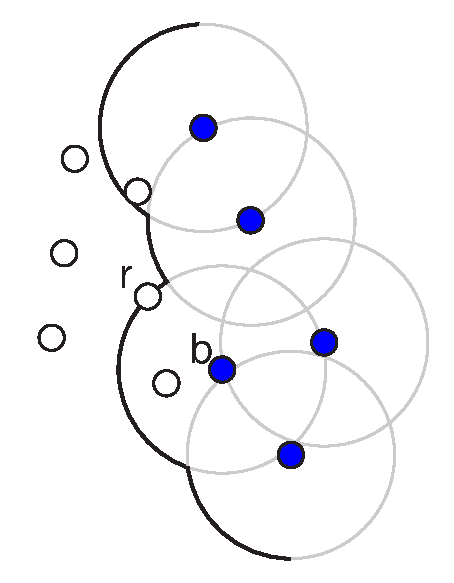
\includegraphics[height=5cm]{biclosest_algorithm}}
  \caption{Left envelope of disks centered at blue points (red
    points are drawn as hollow disks).}
  \label{fig:biclosest_algorithm}
\end{figure}

Algorithm \ref{alg:bichromatic-separated} runs in linear-expected time since
each time through the first while loop, with constant probability, we reduce
the size of $R$ or $B$ by a half.  This algorithm can be implemented using
only a constant amount of extra memory.  In the first while loop, there are
two steps we elaborate on: (1) how to compute and undo the left-envelope, and
(2) how to identify points to the left of the blue envelope. We begin with the
former.

Computing the left-envelope (portions of the disks visible
from the point $(-\infty, 0)$), is very similar to the convex hull
problem and can be solved in \Oh{n} time and \Oh{1} extra memory using an algorithm identical
to Graham's scan since the points are sorted by $Y$-coordinate.  The
implementation of Graham's scan given by Br\"onnimann
\etal~\cite{bronnimann:convex} achieves this with the output being an 
array that contains the elements that contribute to the left envelope
in the first part of the array sorted by $Y$-coordinate and the elements that do not contribute
in the second part of the array. Also, we observe that it is not
particulary difficult to run Graham's scan {\em in reverse} to restore
the $<_y$ sorted order of the elements in \Oh{n} time once we are done
with the left envelope. To see this, consider the following
pseudo-code implementation of Graham's Scan as outlined in \cite{bronnimann:convex}
(Algorithm~\ref{alg:leftHull}):

\begin{algorithm}
  \caption{Computing the left convex hull of a point set.}
  \label{alg:leftHull}
  \begin{algorithmic}[1]
    \REQUIRE All points in the input array $A[0\ldots n-1]$ are sorted according to
    $y$-coordinate.
    \FOR{$i:=0$ to $n-1$}
      \WHILE{$(h \geq 2)$ and 
        (($\texttt{A}[h-2], \texttt{A}[h-1], \texttt{A}[i]$) does not form a right turn)}
        \STATE Set $h:=h-1$.
      \ENDWHILE
      \STATE Swap $\texttt{A}[i]$ and $\texttt{A}[h]$.
      \STATE Set $h=h+1$.
    \ENDFOR
  \end{algorithmic}
\end{algorithm}

The effect of this algorithm can be reversed by
Algorithm~\ref{alg:revertLeftHull}:

\begin{algorithm}
  \caption{Restoring the $<_y$-order after computing the left
    envelope.}
  \label{alg:revertLeftHull}
  \begin{algorithmic}[1]
    \REQUIRE{Array $\texttt{A}[0\ldots h]$ contains the result of running
      Algorithm~\ref{alg:leftHull} on (the sorted) array
      $\texttt{A}[0\ldots n-1]$.}
    \STATE Set $q:=n-1$.
    \WHILE{$h\neq q$}
      \IF{$\texttt{A}[q] <_y \texttt{A}[h]$}
        \STATE Swap $\texttt{A}[h]$ and $\texttt{A}[q]$.
        \STATE Set $q:=q-1$.
        \IF{$\texttt{A}[q] <_y \texttt{A}[h-1]$}
          \STATE Set $h:=h-1$.
        \ENDIF
        \WHILE{($\texttt{A}[h] <_y \texttt{A}[h+1]$) and 
        (($\texttt{A}[h-2], \texttt{A}[h-1], \texttt{A}[i]$) form a right turn)}
          \STATE Set $h:=h+1$.
        \ENDWHILE
      \ELSE
        \STATE Set $h:=h+1$.
      \ENDIF
    \ENDWHILE
  \end{algorithmic}
\end{algorithm}

We now address the problem of determining the red points that are to the left of the blue envelope. To determine whether or not
a given red point $p$ is to the left of the blue envelope, we compute the intersection of a horizontal line through $p$ with the
envelope (see Figure \ref{fig:biclosest_algorithm}). If the intersection point is to the right of $p$ then $p$ is to the left of the envelope.
By scanning the red points from top to bottom and simultaneously scanning the blue envelope from top to bottom, similar to merging
of two sorted lists, all of these intersections can be computed in linear time. We select exactly $\lfloor n/2 \rfloor$ elements of $R$ 
to discard in order to simplify the undo step, similar to what was done in the selection problem.


We now outline how the whole algorithms comes together. We first present the algorithm in standard recursive form.

\begin{algorithm} 
  \caption{Algorithm Bi-Nearest-Neighbor($A,b,e$): Divide-and-Conquer algorithm for finding bi-chromatic closest
    pair.}\label{alg:binn}
  \begin{algorithmic}[1]

    \REQUIRE All points in the input array $A$ are sorted according to
    $X$-coordinate.

    \ENSURE First two points in the array $A[b,\ldots,e]$ realize the
    bi-chromatic closest pair provided $A[b,\ldots,e]$ contains at least
    one red and one blue point and the remaining points are sorted
    according to~$<_Y$.

    \IF{$e-b < 16$}
	 \STATE PROCESS 1: Sort the points according to $Y$-coordinate.
	 If there are at least one red and one blue points, compute
	 a bi-chromatic closest pair using a brute-force algorithm,
	 and stably place them at the front of the current subarray.
    \ELSE
         \STATE PROCESS 2: Stably partition the array based upon the median $X$-coordinate and recurse.
         \STATE Bi-Nearest-Neighbor($A,b,\ldots,\lfloor e/2 \rfloor$)
         \STATE Bi-Nearest-Neighbor($A,\lfloor e/2 \rfloor + 1, e$)
         \STATE PROCESS 3: Record the minimum bi-chromatic closest pair in each of the two subarrays.
         \STATE Let $R_l$ represent the red points in $A[b,\ldots,\lfloor e/2 \rfloor]$.
         \STATE Let $B_r$ represent the blue points in $A[\lfloor e/2 \rfloor + 1,\ldots,e]$.
         \IF{$R_l > 0$ and $B_r > 0$}
               \STATE Compute the Bi-chromatic closest pair for $R_l$ and $B_r$ separated by a line. 
         \ENDIF
         \STATE Let $B_l$ represent the blue points in $A[b,\ldots,\lfloor e/2 \rfloor]$.
         \STATE Let $R_r$ represent the red points in $A[\lfloor e/2 \rfloor + 1,\ldots,e]$.
         \IF{$B_l > 0$ and $R_r > 0$}
               \STATE Compute the Bi-chromatic closest pair for $B_l$ and $R_r$ separated by a line. 
         \ENDIF
         \STATE Compute the minimum of all the bi-chromatic closest pairs.
         \STATE Scan both subarrays such that all points are sorted according to~$<_y$.
         \STATE Stably place the bi-chromatic closest pair to the front of the array.
    \ENDIF
  \end{algorithmic}
\end{algorithm}

Note that this algorithm is similar to Algorithm \ref{alg:nn}. The only steps
we need to elaborate are the steps in PROCESS 3. Prior to Step 10, we use two
invocations to SortedSubsetSelection to move the red points in
$A[b,\ldots,\lfloor e/2 \rfloor]$ and blue points in $A[\lfloor e/2 \rfloor +
1, e]$ to the front of their respective arrays. We use Algorithm
\ref{alg:bichromatic-separated} to compute the closest red-blue pair.  We then
Undo this. Similarly, prior to Step 15, we use two invocations to
SortedSubsetSelection to move the blue points in $A[b,\ldots,\lfloor e/2
\rfloor]$ and red points in $A[\lfloor e/2 \rfloor + 1, e]$ to the front of
their respective arrays, use Algorithm \ref{alg:bichromatic-separated} to
compute the closest pair, followed by an Undo.  Since all the base instances
can be computed in \Oh{n \log n} time and \Oh{1} extra space and each of the
PROCESSES can be computed in \Oh{n} expected time with \Oh{1} extra space, we
conclude with the following:

\begin{theorem}
  Given sets $R$ and $B$ of \orderof{n} points in the plane, a closest
  bichromatic pair can be computed in \Oh{n \log n} expected time
  using \Oh{1} extra memory.
\end{theorem}

We note that if the points $R$ and $B$ are given in separate arrays as input, we can still achieve the same running time using \Oh{1} extra space albeit the 
details become much more tedious. Of course, using \Oh{\log n} extra space is trivial since Algorithm \ref{alg:binn} is in standard recursive form.
%
%\subsection{All Nearest Neighbors}\label{sec:allnn}
%
%In this section, we apply our divide-and-conquer scheme
%to solve the all-nearest neighbors problem space-efficiently. Again,
%we present a modification of Bentley and Shamos' algorithm.
%
%\begin{algorithm}
%  \caption{Divide-and-Conquer algorithm for computing all nearest
%    neighbors~\cite{bentley:divide-and-conquer}.}  
%  \begin{algorithmic}[1]
%    \REQUIRE All points in the input array $A$ are sorted according to
%    $x$-coordinate.
%    \ENSURE All points in $A$ are sorted according to~$<_y$, 
%    and for each point, its nearest neighbor in $A$ is known. 
%    \STATE  If $A$ stores only a constant number of points, sort the
%    points according to $<_y$, compute all nearest neighbors using 
%    a brute-force algorithm, and return.
%    \STATE  Subdivide the array based upon the median
%    $x$-coordinate $x=\ell$ and recurse on both subarrays $A_0$ and
%    $A_1$.  
%    \STATE  Simultaneously scan through both subarrays $A_0$ and $A_1$, and
%    for each point~$p\in A_i$ check all points in $A_{1-i}$ whose
%    nearest-neighbor ball contains the projection of $p$ onto the line
%    $x=\ell$. Update the nearest neighbor information as necessary.
%    \STATE  Merge the points according to $<_y$.
%  \end{algorithmic}
%\end{algorithm}
%
%We can make this algorithm space-efficient using the framework of
%Section 1. One detail, however, needs special attention: Bentley and
%Shamos argue that for each of the points in the sets to be merged,
%only ``a constant number other points needs be
%examined''~\cite[p.~229]{bentley:divide-and-conquer}. More
%specifically, ``this number is four for points in two dimensions under
%the $L_2$ (Euclidean)
%metric''~\cite[p.~228]{bentley:divide-and-conquer}
%
%Note that when processing a point $p$, the four points above and below
%$p$'s $y$-coordinate whose nearest neighbor balls intersect the
%vertical line may be interspersed (with respect to the $<_y$ order) by
%linearly many points. In order to provide constant-time access to
%these points, we proceed as follows. We use $2n \cdot log_2 n$ bits of
%extra space to maintain the following invariants that have to be
%fulfilled as a postcondition after each ``recursive'' call on a
%subarray \texttt{A}$[b \ldots e-1]$, $e > b$:
%
%\begin{description}
%\item[Invariant 1:] $A[b\ldots e-1]$ is sorted according to $<_y$.
%\item[Invariant 2:] Any point $p\in A[b\ldots e-1]$ stores an index
%  $i\in[b\ldots e-1]$ such that $A[i]$ is the nearest neighbor of $p$
%  with respect to $A[b\ldots e-1]$.
%\end{description}
%
%If these invariants are maintained throughout the algorithm, each
%point will store the index of its global nearest neighbor at the end
%of the algorithm. The main problem in performing the merge step of
%this \emph{in-place} version of the divide-and-conquer algorithm is
%that while simultaneously scanning the two sorted arrays of points,
%i.e.  \emph{before} merging them, for each point we need to compute
%the index of its nearest neighbor with respect to the \emph{merged}
%array.
%
%This is done in two phases. First, we do a linear scan to compute the
%index of each element in the merged array and store this index with
%the element (this is where we use $n \cdot log_2 n$ extra bits).
%Next, we perform the merge step, and maintain a look-ahead queue of
%length 8 for each point set. In this queue, we maintain the indices of
%the next 4 and the last 4 points seen whose nearest neighbor balls
%intersect the vertical line at the median $x$-coordinate.  It is easy
%to see that these queues can be maintained space-efficiently while not
%increasing (asymptotically) the running time.
%
%%% Local Variables:
%%% mode: latex
%%% TeX-master: "paper"
%%% End:


%% -*- LaTeX -*- This is LaTeX2e code

\section{Orthogonal line segment intersection}\label{sec:orth}

In this section, we present a space-efficient algorithm for the
orthogonal line segment intersection problem.  Since this problem has
a variable output size $k \in \Oh{n^2}$ we consider the output memory
model to be a write-only space usable only for output and not for
temporary space.  This model has been used by Chen and
Chan~\cite{chen:space-efficient} for variable size output,
space-efficient algorithms and accurately models algorithms that have
output streams with write-only buffer space.

The input to our algorithm is an array $V[0,n-1]$ of $n$ vertical
segments and an array $H[0,m-1]$ of $m$ horizontal segments. The
goal is to output all of the intersections between horizontal and
vertical segments.  Our solution is an algorithm in standard recursive
form. Therefore, we use \Oh{\log n} extra memory and our computation
time is \Oh{n \log n + k} where $k$ is the number of intersections.
This is an improvement over the algorithm by Chen and
Chan\cite{chen:space-efficient}, however they solve the more general
problem of enumerating all intersections among a general set of
line segments.  It is unclear how to convert our solution to
space-efficient recursive form because it is difficult to pre-compute
all of the base instances.  Once we have described the algorithm,
the reason for this difficulty will become clear.



\begin{algorithm}
  \caption{OLSI($V[a,b],H[c,d]$): Report all intersections between vertical line segments in $V[a,b]$ and horizontal line segments $H[c,d]$.} \label{alg:orth}
  \begin{algorithmic}[1]
    \REQUIRE segments in $V$ are sorted by $Y$-coordinate of the top vertices of the segments and segments in $H$ are sorted by $Y$-coordinate.
    \ENSURE all intersections between a segment in $H$ and a segment in $V$ are reported.
    \IF{$b-a$ is 1} 
       \STATE \COMMENT{There are 2 vertical segments in $V[a,b]$.}
       \STATE Let $X_{min}$ be the minimum $X$-coordinate of the segments in $V[a,b]$.
       \STATE Let $X_{max}$ be the maximum $X$-coordinate of all segments in $V[a,b]$.
       \STATE Use \textsc{SortedSubsetSelection}, to select all horizontal segments that completely span the slab $[X_{min},X_{max}]$.
              The segments are placed in $H[c,m_2]$.
       \STATE Scan $V[a,b]$ and $H[c,m_2]$ to report all intersections.
       \STATE UNDO Selection of horizontal segments spanning the slab. We recover $H[c,d]$ from $H[c,m_2]$.
    \ELSE
       \STATE Let $X_{min}$ be the minimum $X$-coordinate of all segments in $V[a,b]$.
       \STATE Let $X_{med}$ be the median $X$-coordinate of all segments in $V[a,b]$.
       \STATE Let $X_{max}$ be the maximum $X$-coordinate of all segments in $V[a,b]$.
       \STATE \COMMENT{$X_{min}$ and $X_{max}$ represent the boundaries of the current vertical slab being processed}.
       \STATE Use \textsc{SortedSubsetSelection}, to select all horizontal segments that completely span the slab $[X_{min},X_{max}]$.
              The segments are placed in $H[c,m_2]$.
              \COMMENT{These are the horizontal segments that are completely spanning the current slab: $[X_{min},X_{max}]$}.
       \STATE Scan $V[a,b]$ and $H[c,m_2]$ to report all intersections.
       \STATE UNDO Selection of horizontal segments spanning the slab. We recover $H[c,d]$ from $H[c,m_2]$.
       \STATE Use \textsc{SortedSubsetSelection} to select all vertical segments in the slab $[X_{min},X_{med}]$.
              The segments are placed in $V[a,m_1]$.
       \STATE Use \textsc{SortedSubsetSelection}, to select all horizontal segments that are in the slab $[X_{min},X_{med}]$ or span the slab $[X_{min},X_{med}]$ but
              DO NOT span the slab $[X_{min},X_{max}]$.
              The segments are placed in $H[c,m_2]$.
       \STATE OLSI($V[a,m_1],H[c,m_2]$).
       \STATE UNDO Selection of horizontal segments to recover $H[c,d]$ from $H[c,m_2]$.
       \STATE UNDO Selection of vertical segments to recover $V[a,b]$ from $V[a,m_1]$.
       \STATE Use \textsc{SortedSubsetSelection} to select all vertical segments in the slab $[X_{med},X_{max}]$.
              The segments are placed in $V[a,m_1]$.
       \STATE Use \textsc{SortedSubsetSelection}, to select all horizontal segments that are in the slab $[X_{med},X_{max}]$ or span the slab $[X_{med},X_{max}]$ but
              DO NOT span the slab $[X_{min},X_{max}]$.
              The segments are placed in $H[c,m_2]$.
       \STATE OLSI($V[a,m_1],H[c,m_2]$).
   \ENDIF
  \end{algorithmic}
\end{algorithm}

The above algorithm is in standard recursive form. Since the recursion tree is balanced, the running time is \Oh{n \log n} 
and the amount of extra memory
required is \Oh{\log n} for the recursion stack. Prior to invoking the recursive algorithm, the segments in $H$ and $V$ are sorted 
in \Oh{n \log n} time. The key point is that an intersection between a horizontal and vertical segment is
reported only when the vertical segment is contained in the current slab and the horizontal segment completely spans the vertical slab.
All of the selection steps and their undo counter-parts are performed using SortedSubsetSelection in linear time with
constant extra memory. Selecting the
segments with maximum and minimum $X$-coordinate in $V[a,b]$ is trivial. Selecting the median can be done in linear expected time with \Oh{1}
extra memory using the algorithm described in Section \ref{sec:sel} or deterministically in linear time and \Oh{1} extra memory using
the algorithm described in Appendix \ref{sec:detkmed}.
The only steps of the algorithm still requiring explanation are Steps 6 and 14: how to report all of the intersections between vertical
segments within a slab and horizontal segments spanning a slab.

Prior to the scan, the vertical segments in $V[a,b]$ are sorted
by $Y$-coordinate of the upper vertices of the segments and the
horizontal segments in $H[c,m_2]$ are sorted by $Y$-coordinate. For
each vertical segment with endpoints $p,q$, we locate the index $i$
in $H$ of the horizontal segment with largest $Y$-coordinate whose
value is at most the $Y$-coordinate of $p$.  Starting at $i$, we
sequentially scan $H$ until we find the index $j$ of the first
horizontal segment whose $Y$-coordinate is more than the $Y$-coordinate
of $q$. Now, all of the segments in $H[i,j-1]$ intersect segment
$pq$. Given $i$, the number of segments of $H$ that are verified
is one more than the number of intersections. A simple scan, similar to the
merging of two sorted lists, shows that all of the $i$'s can be found in linear time.
Since a vertical segment only occurs in \Oh{\log n} slabs, the total amount of time
spent in this step is \Oh{n \log n + k} where $k$ is the number of intersections reports.
We outline the scan below.

\begin{algorithm}
  \caption{Scan($V[a,b],H[c,d]$): Report all intersections between vertical line segments in $V[a,b]$ and horizontal line
           segments in $H[c,d]$.} \label{alg:scan}
  \begin{algorithmic}[1]
    \REQUIRE All vertical segments are within a vertical slab and all the horizontal segments span the slab. All segments in
             $V$ are sorted by $Y$-coordinate of the upper vertex and all segments in $H$ are sorted by $Y$-coordinate.
    \ENSURE all intersections between a segment in $H$ and a segment in $V$ are reported. The order of the segments in $V$ and $H$
            remains unchanged.

\STATE C := a \COMMENT{C represents the index of the current vertical segment}.
\STATE T := index of first $Y$-coordinate in $H[c,d]$ that is smaller than $Y$ coordinate of $V[C]$.
\STATE R := T.
\WHILE{$C \leq b$}
      \WHILE{$Y$-coordinate of $H[R] > Y$-coordinate of $V[C]$}
            \STATE Report intersection and increment R by 1.
      \ENDWHILE
      \STATE increment C by 1.
      \STATE update T and set $R: = T$. 
\ENDWHILE

  \end{algorithmic}
\end{algorithm}


%% state theorem
\begin{theorem}
Given a set of $n$ vertical line segments in an array $V$ and a set of $m$ horizontal line segments in an array $H$, all
intersections between horizontal and vertical segments can be reported in \Oh{(n + m)\log n + k} time using \Oh{\log n} extra space where $k$ is
the number of intersections reported.
\end{theorem}

The main difficutly in transforming this algorithm into space-efficient recursive form stems from the difficulty of pre-computing
all of the base instances. Since a horizontal line segment can span a logarithmic number of slabs, we are unable
to precompute the base instances in a simple way.


%%% Local Variables:
%%% mode: latex
%%% TeX-master: "paper"
%%% End:


%%% -*- LaTeX -*- This is LaTeX2e code

\section{Other Space-Efficient Geometric Algorithms}

In this section, we present some simple observations about well-known
algorithms for three geometric problems and show how to space-efficiently
encode the results.

\subsection{Convex Hull of a Simple Polygon}

Using an space-efficient stack, e.g., along the lines of Br\"onnimann
\etal\'{}s~\cite{bronnimann:convex} description of Graham\'{}s
Scan~\cite{graham:efficient}, we can implement an optimal
space-efficient algorithm for computing the convex hull of a simple
polygon. To do so, we only need to observe that the only operations
performed in the algorithm described by Preparata and
Shamos~\cite[Chap. 4.1.4]{preparata:computational} are push and pop
operations.

\begin{lemma}
  The convex hull of a simple polygon with $n$ vertices can
  be computed \emph{in-place} in \Oh{n} time.
\end{lemma}

\subsection{Diameter of a Point Set}

Using the space-efficient algorithm of Br\"onnimann
\etal~\cite{bronnimann:convex}, we immediately obtain an optimal
space-efficient algorithm for computing the diameter of a point set.
This is due to the fact that the algorithm for enumerating antipodal
pairs as described by Preparata and
Shamos~\cite[Chap. 4.2.3]{preparata:computational} already is an
\emph{in-place} traversal of the boundary of the convex hull. To
encode the output without any extra space, we use an \emph{in-place}
partitioning algorithm, e.g. \cite{katajainen:partitioning}, to move
an antipodal pair determining the diameter to the start of the array
containing the points.

\begin{lemma}
  The diameter of a set of $n$ points in the plane can be computed
  \emph{in place} in \Oh{n \log_2 n} time. The encoding of the result
  does not need any extra space.
\end{lemma}

\subsection{Minimum Enclosing Circle}

A close look at Welzl\'{}s incremental
algorithm~\cite{welzl:smallest} shows that this algorithm already
works \emph{in-place}. We can modify the output of this algorithm such
that the array containing the points is reorganized in the following
way: Either the first three points determine the minimum enclosing
circle or the first two points determine the diameter of the circle.
Which of these cases applies, can be checked by first assuming that
the first two points determine the diameter and then checking whether
the third point is contained within this circle. As we can always
arrange the three points that determine the minimum enclosing circle
in such a way that the circle given by first two points does not
contain the third point (take the endpoints of the shortest edge in
the triangle formed by these points), this shows that the result
can be encoded without any extra space.

\begin{lemma}
  The Minimum Enclosing Circle of a set of $n$ points in the plane can
  be computed \emph{in-place} in \Oh{n} expected time. The encoding of
  the result does not need any extra space.
\end{lemma}

%%% Local Variables:
%%% mode: latex
%%% TeX-master: "paper"
%%% End:

%% -*- LaTeX -*- This is LaTeX2e code



\section{Conclusions}\label{sec:conc}
In this paper, we presented a number of space-efficient tools. In
particular, we presented a scheme for transforming a recursive
function in standard form to one in space-efficient form reducing
the amount of extra memory used to traverse the recursion tree.  We
provided a simple way to stably select a set of elements within an
ordered array, and {\em undo-ing} the stable selection.  We also
provided a tool for easily selecting in linear time with constant
extra space, the $k$-th smallest element in one dimension from an
array of points in $2$ or more dimensions when the points are sorted
in another dimension.  All of these tools are applied to solve
several geometric problems that have solutions using some form of
divide-and-conquer. Specifically, we address the problem of nearest
neighbor, bichromatic nearest neighbor and orthogonal line segment
intersection.

We conclude with two open problems. First, can one
devise a deterministic counter-part to the randomized algorithm presented
for computing the bi-chromatic closest pair for points separated by a vertical line?
Second, is it possible to solve the orthogonal line segment intersection problem
with only $O(1)$ extra memory?

%%% Local Variables:
%%% mode: latex
%%% TeX-master: "paper"
%%% End:


\bibliographystyle{abbrv}
\bibliography{allrefs}

\begin{appendix}
  %% -*- LaTeX -*- This is LaTeX2e code

\newcommand{\LA}{\ensuremath{<_{y}}}
\newcommand{\LB}{\ensuremath{<_{x}}}

\section{Selecting the $k$-th smallest element} \label{sec:detkmed}

In this appendix, we describe a space-efficient variant of the
well-known median-find algorithm by Blum \etal~\cite{blum:selection}.
Our algorithm assumes that the input is given in the form of an array
${A}[0\ldots n-1]$ which is sorted according to some total
order \LA. The goal of the algorithm is, given an integer $k\in
[0\ldots n-1]$, to select the $k$-th smallest element in {A}
\emph{according to some other total order} \LB. This algorithm will
run in linear time and will require only \Oh{1} extra space. 
Additionally, the algorithm returns the array ${A}[0\ldots n-1]$ 
in the same order as it was presented, namely sorted according to \LA.

The correctness of the algorithm described below will follow from the
following invariant:

\begin{description}
\item[Invariant:] Assume the algorithm is called to select the $k$-th
  smallest element from a \LA-sorted (sub-)array
  ${A}[b\ldots e-1]$, where $b,e$, and $k$, are three global
  variables. Then, upon returning from this call, $b,e$, and $k$ 
  have been restored to the values they had when the algorithm was 
  called. Additionally, ${A}[b\ldots e-1]$ is sorted according 
  to \LA. 
\end{description}


\newcounter{ALGBREAK}
\newcounter{SelectA}
\newcounter{SelectB}
\newcounter{SelectC}
\newcounter{StackA}
\newcounter{StackB}

\begin{algorithm}
  \caption{The algorithm
    $\textsc{RestoringSelect}({A},b,e,k,\text{mode})$ for
    selecting the $k$-th smallest element in ${A}[b\ldots
    e-1]$ (if $\text{mode}=\textsc{Select}$) or the median element (if
    $\text{mode}=\textsc{Median}$).}
  \begin{algorithmic}[1]
    \REQUIRE ${A}[b\ldots e-1]$ is sorted according to
    \LA. 
    \ENSURE ${A}[b\ldots e-1]$ is sorted according to
    \LA. The variables $b,e$, and $k$ are reset to their
    original values. 
    \STATE Subdivide ${A}[b\ldots e-1]$ into $\lfloor(e-b)/5
    \rfloor$ groups of $5$ elements and (possibly) one group of size 
    $\leq 4$.  
    \STATE Move the medians of the first $\lfloor(e-b)/5 \rfloor$ 
    groups to ${A}[b\ldots b+\lfloor(e-b)/5\rfloor-1]$ using 
    algorithm \textsc{SortedSubsetSelection}.  
    \STATE $i \leftarrow (e-b) - \lfloor(e-b)/5\rfloor\cdot 5$
    \STATE $\textsc{Push}(S,i)$ \setcounter{StackA}{\value{ALC@line}}
    \STATE
    $i_{\mathrm{med}} \leftarrow 
       \textsc{RestoringSelect}({A},b,b+\lfloor(e-b)/5\rfloor,k,\textsc{Median})$
    \setcounter{SelectA}{\value{ALC@line}}
    \STATE
    $\textsc{UndoSubsetSelection}({A},b,b+\lfloor(e-b)/5\rfloor\cdot 5, \lfloor(e-b)/5\rfloor)$
    \STATE $i \leftarrow \textsc{Pop}(S)$ \setcounter{StackB}{\value{ALC@line}}
    \STATE $e \leftarrow b + \lfloor(e-b)/5\rfloor \cdot 5 + i$
    \IF{$\text{mode} = \textsc{Median}$}
      \STATE $l \leftarrow \lfloor (e-b)/2 \rfloor$
    \ELSE
      \STATE $l \leftarrow k$
    \ENDIF
    \STATE $x \leftarrow {A}[i_{\mathrm{med}}]$
    \STATE 
     $k_< \leftarrow |\left\{a\in{A}[b\ldots e-1] \mid a<x\right\}|$
    \STATE 
     $k_= \leftarrow |\left\{a\in{A}[b\ldots e-1] \mid a=x\right\}|$ 
    \STATE 
     $k_> \leftarrow |\left\{a\in{A}[b\ldots e-1] \mid a>x\right\}|$
    \IF{$l\notin [k_< + 1, k_< + k_=]$}
      \IF{$l \leq k_<$}
        \IF{$l = k_<$}
          \STATE Set $i_{\mathrm{med}}$ to point to the largest element
          in ${A}[b\ldots e-1]$ less than $x$ (according to \LB).
        \ELSE
          \STATE Move $x$ to ${A}[b]$.
          \STATE Using \textsc{SortedSubsetSelection}, move all elements in
          ${A}[b+1\ldots e-1]$ less than $x$ to
          ${A}[b+1\ldots b+k_<]$.
          \STATE Move the largest element less than $x$ (according to
          \LB) to ${A}[e-1]$ .
          \STATE
          $i_{\mathrm{med}} \leftarrow 
            \textsc{RestoringSelect}({A},b+1,b+k_<,k,\textsc{Select})$
          \setcounter{SelectB}{\value{ALC@line}}
          \STATE Starting at ${A}[b+k_<]$, scan ${A}$ to find
          $e-1$ (the index of the first element $y$ for which 
          $y\LB x:=A[b]$). 
          \STATE Move ${A}[e-1]$ to its proper position in
          ${A}[b+1\ldots b+k_<]$.
          \STATE $\textsc{UndoSubsetSelection}({A},b+1,e,b+k_<+1)$.
          \STATE Reinsert (according to \LA) $x:={A}[b]$ into
          ${A}[b\ldots e-1]$ maintaining $i_{\mathrm{med}}$.
        \ENDIF
          \setcounter{ALGBREAK}{\value{ALC@line}}
       \ELSE
         \STATE (\ldots) \\[2ex]
         \setcounter{ALC@line}{44}
       \ENDIF
     \ENDIF
     \STATE Return $i_{\mathrm{med}}$.
 \end{algorithmic}
\end{algorithm}

\begin{algorithm}
  \addtocounter{algorithm}{-1}
  \caption{Algorithm
    $\textsc{RestoringSelect}({A},b,e,k,\text{mode})$ (contd.)}
  \begin{algorithmic}[1]
    \setcounter{ALC@line}{17}
    \IF{$l\notin [k_< + 1, k_< + k_=]$}
      \IF{$l \leq k_<$}
        \STATE (\ldots)\\[2ex]
        \setcounter{ALC@line}{\value{ALGBREAK}}
      \ELSE
        \IF{$l = b-e$}
          \STATE Set $i_{\mathrm{med}}$ to point to the largest element
          in ${A}[b\ldots e-1]$ larger than $x$ (according to \LB).
        \ELSE
          \STATE Using \textsc{SortedSubsetSelection}, move all elements in
          ${A}[b+1\ldots e-1]$ larger than $x$ to
          ${A}[b+1\ldots b+k_>]$.
          \STATE Move the smallest element larger than $x$ (according to
          \LB) to ${A}[e-1]$.
          \STATE
          $i_{\mathrm{med}} \leftarrow 
           \textsc{RestoringSelect}({A},b+1,b+k_>,k-(k_<+k_=),\textsc{Select})$.
          \setcounter{SelectC}{\value{ALC@line}}
          \STATE Starting at ${A}[b+k_>]$, scan ${A}$ to find
          $e-1$ (the index of the first element $y$ for which 
          ${A}[b] =: x <_{x} y$). 
          \STATE Move ${A}[e-1]$ to its proper position in
          ${A}[b+1\ldots b+k_>]$.
          \STATE $\textsc{UndoSubsetSelection}({A},b+1,e,b+k_>+1)$.
          \STATE Reinsert (according to \LA) $x:=A[b]$ into
          ${A}[b\ldots e-1]$ maintaining $i_{\mathrm{med}}$.
          \STATE Recompute $k_<$ and $k_=$ (as above) and set 
            $k \leftarrow (k-(k_<+k_=))+k_<+k_=$. 
        \ENDIF
       \ENDIF
    \ENDIF
    \STATE Return $i_{\mathrm{med}}$.
  \end{algorithmic}
\end{algorithm}

The invariant is to enforce trivially for any constant-sized input. 
Algorithm~13 is described in a recursive way to facilitate the 
analysis and the proof of correctness. We can convert this algorithm 
into a non-recursive variant by simply maintaining a stack of 
two-bit entries that indicate whether the current ``invocation'' took 
place from line \theSelectA, \theSelectB, or \theSelectC. This stack 
has a worst-case depth of \Oh{\log n} and thus will (in an asymptotic 
sense) not increase the extra space required by this algorithm. 
Also, the stack $S$ used in lines \theStackA\ and \theStackB\ 
contains only integers in the range $[0\ldots 4]$, so its overall 
size is bounded by \Oh{\log n} bits,
too. 

Assuming that the above invariant is fulfilled for any constant-size
input, we can inductively assume that the invariant holds after the
``recursive'' call in line~\theSelectA. This implies that for the
successive call to \textsc{UndoSubsetSelection} the parameters $b$,
$\lfloor(e-b)/5\rfloor$, and hence also $e_1:=b+\lfloor(e-b)/5\rfloor$
and $e_2:=b+\lfloor(e-b)/5\rfloor\cdot 5$ are known. The situation
prior to the call to \textsc{UndoSubsetSelection} is depicted in
Figure~\ref{fig:undomedian}: The array ${A}[b\ldots e_1-1]$
contains the medians in sorted \LA-order that had been
selected from ${A}[b\ldots e_2-1]$, and the remaining $i$
elements are still untouched, hence also sorted according to
\LA. 

\begin{figure}[ht]
  \renewcommand{\arraystretch}{1.75}
  \begin{center}
  \begin{tabular}{cccrrcrl}
    \hline
    \ldots & 
    \multicolumn{2}{|c|}{medians \LA-sorted} &
    \multicolumn{2}{c|}{unsorted} &
    \multicolumn{2}{c|}{rest \LA-sorted} & 
    \ldots \\
    \hline 
    &
    {\small $b$} &
    &
    {\small $e_1$} & 
    &
    {\small $e_2$} & 
    &
    {\small $e_2+i$} 
  \end{tabular}
  \end{center}
  \caption{Restoring the \LA-order after having computed
    the median of the $\lfloor(b-e)/5\rfloor$ medians. 
    Here $e_1:= b + \lfloor(b-e)/5\rfloor$ and  
    $e_2:= b + \lfloor(b-e)/5\rfloor \cdot 5$.}
  \label{fig:undomedian}
\end{figure}

As a consequence, we can first undo the effects of
\textsc{SortedSubsetSelection} on ${A}[b\ldots e_2 -1]$, hence
restoring it to sorted \LA-order and finally adjust $e$
to point to $e_2 + i$. This implies that $b$ and $e$ are known and
${A}[b\ldots e-1]$ is sorted according to \LA. As the original
value of $k$ had been passed to the ``recursive'' call to
\textsc{RestoringSelection}, by the invariant, we still know its value.

For the second and third situtation in which a ``recursive'' call to
\textsc{RestoringSelection} may happen (lines \theSelectB\ and
\theSelectC), we do not know how many elements are passed to
the ``recursive'' call. In order to recover the original value of
$e$ after the call, we move the median-of-medians $x$ to the front of
the array and use a distinguished element $y$ to denote the \emph{end}
of the subarray that is not passed to the recursive call. Let us 
consider the situation where the $k$-th element to be selected is 
larger (according to \LB) than the median-of-medians $x$ (the other 
situation is handled analogously). Prior to the ``recursive'' call 
in line \theSelectC\ we have moved all elements larger than $x$ to 
the front of the array, more specifically to the subarray 
${A}[b+1\ldots b+k_>]$. Then we find the largest element 
larger than $x$ (using a single scan) and move it to the end of the 
current array ${A}[b\ldots e-1]$. This element, being larger 
than $x$, is also larger than any element not passed to the 
``recursive'' call and will be the first element larger than $x$ 
encountered when scanning the array ${A}$ starting from 
${A}[b+k_>]$ (Figure~\ref{fig:undoselect}).

\begin{figure}[ht]
  \renewcommand{\arraystretch}{1.75}
  \begin{center}
  \begin{tabular}{ccccrrcl}
    \hline
    \ldots & 
    \multicolumn{1}{|c}{$x$} &
    \multicolumn{2}{|c|}{``$x$ \LB'' \LA-sorted} &
    \multicolumn{2}{c|}{``$x \not<_{x}$'' unsorted} &
    \multicolumn{1}{c|}{$y$} & 
    \ldots \\
    \hline 
    &
    {\small $b$} &
    {\small $b+1$} &
    &
    {\small $b+k_>$} & 
    & {\small ?}
    & {\small $e$}
  \end{tabular}
  \end{center}
  \caption{Restoring the \LA-order after having selected the
    $k-(k_<+k_=)$-th element from ${A}[b+1\ldots b+k_>-1]$.
    Here $y$ is the largest element in ${A}[b\ldots e-1]$ for
    which $x\LB y$.}
  \label{fig:undoselect}
\end{figure}

By the invariant, we know that after the ``recursive call'' to
\textsc{RestoringSubsetSelection}$({A},b+1,b+k_>,k-(k_<+k_=)$,
the subarray ${A}[b+1\ldots b+k_>-1]$ will be sorted according
to \LA, and we will know the values of $b+1$, $b+k_>$, and
$k-(k_<+k_=)$. This enables us to retrieve the median-of-medians $x$
from ${A}[b]$ and (starting from ${A}[b+k_>]$) to scan
for the first element larger than $x$. After we have found this
element at position $e-1$, we have restored to original value of $e$,
and a single scan over ${A}[b\ldots e-1]$ allows us to
compute the values $k_<$ and $k_=$, which are needed to restore $k$ to
its original value. 

Inductively, we see that the invariant holds for the initial call to
the algorithm, and this implies that the algorithm selects the $k$-th
smallest element according to \LB\ while maintaining the \LA-order in
which the elements had been given. The space requirement of this
algorithm is \Oh{\log n} bits, because besides a constant number of
indices, only two stacks of size \Oh{\log n} bits are needed. Using
the analysis of the original algorithm by Blum 
\etal~\cite{blum:selection}, the running time can be shown to be
\Oh{n}, and we conclude with the following theorem:

\begin{theorem}\label{lem:select}
 The $k$-th smallest element in an array of $n$ element can be 
 selected in linear time using \Oh{1} extra space. Furthermore, if 
 the set is given sorted according to some total order, this order 
 can be restored in the same time and space complexity.
\end{theorem}

%%% Local Variables:
%%% mode: latex
%%% TeX-master: "paper"
%%% End:

  %% -*- LaTeX -*- This is LaTeX2e code


\newcommand{\LU}{\ensuremath{<_{y.\mathrm{upper}}}}
\newcommand{\LY}{\ensuremath{<_{y}}}

\section{Orthogonal Line-Segment Intersection}\label{sec:olsi}

In this appendix, we describe an algorithm that solves the
orthogonal line segment intersection problem in
\Oh{n \log n +k} time using \Oh{1} extra space, where $n$
is the total number of line segments and $k$ is the total number
of intersections. We assume that the input is given in the form
of two arrays ${H}[0\ldots n_h-1]$ and
${V}[0\ldots n_v-1]$ of horizontal and vertical line
segments, respectively, where $n = n_h + n_v$.

We will describe the algorithm as a recursive algorithm. Since it
follows the general framework of Section~\ref{sec:tools}, however, we
can make it space-efficient so that it uses only \Oh{1} extra space.

Consider a subarray ${V}[0\ldots e_v-1]$, and let
$m:=2^{\lfloor \log_2 ((e_v)/2) \rfloor}$. Let $i$ be the index
such that the $X$-coordinate of $V[i]$ is the $m$-th smallest among
all $X$-coordinates of the line segments in this subarray.
Our algorithm will use $V[i]$ to first partition the subarray into a
subarray of length $m$ (we call this ``partitioning the left'') and then
into a subarray of length $e_v-m$ (we call this ``partitioning
the right''). These partitioning algorithms are given as
Algorithms~\ref{algPreVP} and~\ref{algMidVP}. Both of them can be 
undone, see Algorithms~\ref{algUndoPreVP} and~\ref{algUndoMidVP}. 

\begin{algorithm}

  \caption{\textsc{PreVerticalPartition}(${V}$,$e_v$) Partition
  the vertical segments before the first recursive call (Partitioning
  the left)}
  
  \label{algPreVP}
  \begin{algorithmic}[1]
    \REQUIRE ${V}[0\ldots e_v-1]$ is sorted according to
    \LU, i.e., $Y$-coordinates of the upper endpoints. 
    \ENSURE That $e_v:=m$ and the resulting array 
    ${V}[0\ldots e_v-1]$ contains all vertical segments not to the 
    right of the $X$-median, and is sorted according to \LU. 
    \STATE $m \leftarrow 2^{\lfloor \log_2 ((e_v)/2) \rfloor}$
    %% \COMMENT{$m=e_v/2 \iff e_v\neq |V|$}
    \STATE $i \leftarrow 
           \textsc{RestoringSelect}({V},0,e_v,m,\textsc{Select})$. 
    \STATE Using \textsc{SortedSubsetSelection}, move all elements
    less than or equal to ${V}[i]$ to ${V}[0\ldots m-1]$.
    \STATE $\textsc{Push}(S,\textsc{Left})$.
    \STATE $e_v \leftarrow m$
    \STATE Return $e_v$
 \end{algorithmic}
\end{algorithm}

\begin{algorithm}

  \caption{\textsc{UndoPreVerticalPartition}(${V}$,$e_v$)
  Undo the pre-partitioning of the vertical segments after returning
  from the first recursive call.}
  \label{algUndoPreVP}
  \begin{algorithmic}[1]
    \REQUIRE The first recursion has ended, and we are given an array 
    ${V}[0\ldots e_v-1]$ that is sorted according to \LU.
    \ENSURE  The variable $e_v$ has been reset to its original value and 
    the resulting array ${V}[0\ldots e_v-1]$ is sorted 
    according to \LU.
    \STATE $\textsc{Pop}(S)$.
    \IF{$2e_v \leq |V|$}
      \STATE $e_v^{orig} \leftarrow 2e_v$.
    \ELSE
      \STATE $e_v^{orig} \leftarrow |V|$.
    \ENDIF
    \STATE $\textsc{UndoSubsetSelection}({V},0,e_v^{orig},e_v)$
    \STATE $e_v \leftarrow e_v^{orig}$
    \STATE Return $e_v$
 \end{algorithmic}
\end{algorithm}

\newcounter{RestoreRight}

\begin{algorithm}
  \caption{\textsc{MidVerticalPartition}(${V}$,$e_v$) Partition
  the vertical segments before the second recursive call.} 
  \label{algMidVP}
  \begin{algorithmic}[1]
    \REQUIRE ${V}[0\ldots e_v-1]$ is sorted according to \LU.
    \ENSURE That $e_v := e_v - m$ and that the resulting array 
    ${V}[0\ldots e_v]$ contains all vertical segments to the right of 
    the $X$-median and is sorted according to \LU.
    \STATE $m \leftarrow 2^{\lfloor \log_2 (e_v/2) \rfloor}$
    %% \COMMENT{$m=e_v/2 \iff e_v\neq |V|$}
    \STATE $i \leftarrow 
         \textsc{RestoringSelect}({V},0,e_v,m,\textsc{Select})$. 
    \STATE Using \textsc{SortedSubsetSelection}, move all elements
    larger than ${V}[i]$ to ${V}[0\ldots e_v - m-1 ]$.
    \STATE $\textsc{Push}(S,\textsc{Right})$.
    \STATE $e_v \leftarrow e_v-m$
    \STATE Return $e_v$
 \end{algorithmic}
\end{algorithm}

\begin{algorithm}

  \caption{\textsc{UndoMidVerticalPartition}(${V}$,$e_v$)
  Undo the partitioning of the vertical segments after returning from
  the second recursive call}
  \label{algUndoMidVP}
   
  \begin{algorithmic}[1]
    \REQUIRE The last recursive call has ended, and we are
    given an array ${V}[0\ldots e_v]$ that is
    sorted  according to \LU.
    \ENSURE The variable $e_v$ has been reset to its original value and 
    the resulting array ${V}[0\ldots e_v-1]$ is sorted 
    according to \LU.  
    \STATE $\textsc{Pop}(S)$.
    \STATE Let $d$ be the number of elements on the stack $S$.
    \STATE $e_v^{orig} \leftarrow 2^{\lceil\log_2 |V|\rceil - (d+1)} +
    e_v$. \setcounter{RestoreRight}{\value{ALC@line}} 
    \STATE $\textsc{UndoSubsetSelection}({V},0,e_v^{orig},e_v)$
    \STATE $e_v \leftarrow e_v^{orig}$
    \STATE Return $e_v$
 \end{algorithmic}
\end{algorithm}

The observation that shows the correctness of the formula for
restoring the value of $e_v$ (Line~\theRestoreRight\ in 
Algorithm~\ref{algUndoMidVP}) is that the left
subtree of the current node is a complete binary tree. The height of
the tree is the height of the recursion tree (which is $\lceil\log_2
|V|\rceil$) minus the depth of the current node.
%% , that is minus the depth of the ``recursion'' at present. 
The number of leaves in the
left subtree, and hence the number of elements on which the first 
recursive call took place, is then $2^{\lceil\log_2 |V|\rceil -
  (d+1)}$, which is also the index of the split point.

\newcounter{StopElement}
\begin{algorithm}
  \caption{\textsc{PreHorizontalPartition}(${H}$,$e_h$)
  Partition the horizontal segments before the first recursive call.} 
   \label{algPreHP}
  \begin{algorithmic}[1]
    \REQUIRE ${H}[0\ldots e_h-1]$ is sorted according to
    \LY. The current slab boundaries as well as the median for
    splitting the slab are known.
    \ENSURE That $e_h := m$ and the resulting array 
    ${H}[0\ldots e_h-1]$ contains all horizontal segments to be 
    passed to the first recursion sorted according to \LY.
    \STATE Let $m$ be the number of elements in ${H}[0\ldots
    e_h-1]$ that intersect the left sub-slab and do not cross the
    current slab.
    \IF{$m < e_h$}
      \STATE $\textsc{Push}(T,1)$. \COMMENT{At least one segment will not
        move.}
      \STATE Synchronously go back in stack $T$ and stack $S$ and find
      the most recent recursion (except for the current) where at
      least one segment was not moved. Let $R$ be the type of this
      recursion. 
      \IF{$R=\textsc{Right}$}
        \STATE Let $h$ be the segment of those crossing the current
        slab with the leftmost left endpoint. 
      \ELSE
        \STATE Let $h$ be the segment of those crossing the current
        slab with the rightmost right endpoint. 
      \ENDIF
      \IF{$h$ is undefined}
        \STATE Let $h$ be ${H}[m]$. \COMMENT{Don't do anything.}
      \ENDIF
      \STATE Move $h$ to ${H}[m]$. \setcounter{StopElement}{\value{ALC@line}}
      \STATE Using \textsc{SortedSubsetSelection}, move all elements
      except for those that (a) avoid the left sub-slab or (b)
      cross the current slab to ${H}[0\ldots m-1]$. 
    \ELSE
      \STATE $\textsc{Push}(T,0)$.
    \ENDIF
    \STATE $e_h \leftarrow m$
    \STATE Return $e_h$
 \end{algorithmic}
\end{algorithm}

\begin{algorithm}

  \caption{\textsc{UndoPreHorizontalPartition}(${H}$,$e_h$)
  Undo the partitioning of the horizontal segments after returning from
  the first recursive call.} 
    \label{algUndoPHP}
    
  \begin{algorithmic}[1]
    \REQUIRE The first recursive call has ended, and we are
    given an array ${H}[0\ldots e_h-1]$ that is
    sorted  according to \LY. The current slab boundaries as well as
    the median for splitting the slab is known.
    \ENSURE The variable $e_h$ have been reset to its original value and
    the resulting array ${H}[0\ldots e_h-1]$ is sorted 
    according to \LY. 
    \STATE $i \leftarrow \textsc{Pop}(T)$.
    \IF{$i=0$}
      \STATE \COMMENT{No partitioning needs to be reverted.}
    \ELSE
      \STATE $h \leftarrow {H}[e_h]$.
      \IF{$h$ crosses the current slab}
        \STATE Synchronously go back in stack $T$ and stack $S$ and find
        the most recent recursion (except for the current) where at
        least one segment was not moved. Let $R$ be the type of this
        recursion. 
        \IF{$R=\textsc{Right}$}
          \STATE Starting at ${H}[e_h+1]$, scan to find the first
          element that either is right of the current slab or which
          crosses the current slab and whose left endpoint is left of
          $h$'s left endpoint.  
        \ELSE
          \STATE Starting at ${H}[e_h+1]$, scan to find the first
          element that either is right of the current slab or which
          crosses the current slab and whose right endpoint is right of
          $h$'s right endpoint. 
        \ENDIF
      \ELSE
        \STATE Starting at ${H}[e_h+1]$, scan to find the
        first element whose right endpoint is right of the right slab
        boundary or the first element which crosses the current slab.
      \ENDIF
      \STATE Let $e_h^{orig}$ be the index of the element just found.
      \STATE $\textsc{UndoSubsetSelection}({H},0,e_h^{orig},e_h)$
      \STATE Move $h$ to its proper position.
      \STATE $e_h \leftarrow e_h^{orig}$
      \STATE Return $e_h$
    \ENDIF
 \end{algorithmic}
\end{algorithm}

After a subarray ${V}[0\ldots e_v-1]$ has been ``partitioned
to the left'', the vertical slab spanned by
${V}[0\ldots e_v-1]$ (this is the \emph{current slab})
has been partitioned into a \emph{left sub-slab} and a
\emph{right sub-slab}. At this moment, we use these sub-slabs to
partition the corresponding subarray ${H}[0\ldots e_h-1]$
of horizontal line segments. To be more precise, in ``partitioning the 
left'' (see Algorithm~\ref{algPreHP}), the initial part 
of the subarray of ${H}$ contains all $m$ horizontal line segments
in the subarray that intersect the left sub-slab and do not cross the
current slab. A problem arises when we want to undo this partitioning
(in Algorithm~\ref{algUndoPHP}): At that moment, we do not know the 
original value of $e_h$. The solution is to store a ``special'' horizontal 
segment (\emph{viz}.\ the segment $h$ in Line~\theStopElement\ 
of Algorithm~\ref{algPreHP}) in ${H}[m]$.

This segment is used to distinguish horizontal segments crossing the
left sub-slab from horizontal segments crossing a slab corresponding
to a recursive call higher up in the recursion tree. These segments
may be stored in cells ${H}[m]$ and higher and may make it
impossible to re-obtain the original index $e_h$ that is needed in the
restoration process. If there is no segment crossing the current
slab, but at least one segment did not move, we can easily re-obtain
the original index $e_h$ by searching for the first segment that is either
to the right of the current slab or completely crosses the current
slab.

Because of the special role of the horizontal line segment $h$,
we use a variant of \textsc{SortedSubsetSelection} in
Algorithm~\ref{algPreHP} and a variant of \textsc{UndoSubsetSelection}
in Algorithm~\ref{algUndoPHP}. These variants skip over the line 
segment $h$. 
%entry
%${H}[e_h]$.

We have only described how to partition the subarray
${H}[0\ldots e_h-1]$ ``to the left''.
In a completely symmetric way, this subarray can be partitioned
``to the right''.

Having these subroutines at hand, the algorithm solving the orthogonal 
line segment intersection problem is given as Algorithm~\ref{algIOLSI}.

\begin{algorithm}

  \caption{\textsc{ImprovedOLSI}(${V}$,$e_v$,${H}$,$e_h$)
  Solving the Orthogonal Line Segment Intersection Problem.} 
   \label{algIOLSI}
  
  \begin{algorithmic}[1]
    \STATE Scan ${V}[0\ldots e_v-1]$ to compute the
    boundaries of the current slab (min/max values of
    $X$-coordinates). 
    \STATE Using \textsc{SortedSubsetSelection}, move all horizontal 
    segments spanning the current slab to ${H}[0\ldots \ell -1]$. 
    \STATE Perform a top-down sweep over ${H}[0\ldots \ell -1]$
    and ${V}[0\ldots e_v-1]$ to find all intersections.
    \STATE \textsc{UndoSubsetSelection} on
    ${H}[0\ldots e_h-1]$.
    \STATE $e_v \leftarrow$ \textsc{PreVerticalPartition}(${V}$,$e_v$)
    \STATE $e_h \leftarrow$ \textsc{PreHorizontalPartition}(${H}$,$e_h$)
    \STATE \textsc{ImprovedOLSI}(${V}$,$e_v$,${H}$,$e_h$)
    \STATE $e_v \leftarrow$ \textsc{UndoPreVerticalPartition}(${V}$,$e_v$)
    \STATE \textsc{UndoPreHorizontalPartition}(${H}$,$e_h$,$m_h$)
    \STATE $e_v \leftarrow$ \textsc{MidVerticalPartition}(${V}$,$e_v$)
    \STATE $e_h \leftarrow$ \textsc{MidHorizontalPartition}(${H}$,$e_h$)
    \STATE
    \textsc{ImprovedOLSI}(${V}$,$e_v$,${H}$,$e_h$)
    \STATE $e_v \leftarrow$ \textsc{UndoMidVerticalPartition}(${V}$,$e_v$)
    \STATE $e_h \leftarrow$ \textsc{UndoMidHorizontalPartition}(${H}$,$e_h$)
  \end{algorithmic}
\end{algorithm}

\begin{theorem}
Given a set of $n$ horizontal and vertical line segments, all $k$ 
intersections among them can be reported in \Oh{n\log n + k} time 
using \Oh{1} extra space. 
\end{theorem}


%%% Local Variables:
%%% mode: latex
%%% TeX-master: "paper"
%%% End:

\end{appendix}

\end{document}
